\documentclass{article}

\usepackage[spanish]{babel}
\usepackage[numbers,sort&compress]{natbib}
\usepackage{graphicx}
\usepackage{url}
\usepackage{amsmath}
\usepackage{hyperref}
\usepackage{listings}
\usepackage[top=30mm, bottom=40mm, left=15mm, right=15mm]{geometry}
\usepackage{color}
\usepackage{subfig}
\usepackage{float}
 
\definecolor{codeblue}{RGB}{0,128,255}
\definecolor{codegray}{rgb}{0.5,0.5,0.5}
\definecolor{codepurple}{rgb}{0.58,0,0.82}
\definecolor{pink}{RGB}{255,26,117}
\definecolor{backcolour}{rgb}{1,1,1}
 
\lstdefinestyle{mystyle}{
    backgroundcolor=\color{backcolour},
    commentstyle=\color{codeblue},
    keywordstyle=\color{pink},
    numberstyle=\tiny\color{codeblue},
    stringstyle=\color{codepurple},
    basicstyle=\footnotesize,
    breakatwhitespace=false,         
    breaklines=true,                 
    captionpos=b,                    
    keepspaces=true,                 
    numbers=left,                    
    numbersep=7pt,                  
    showspaces=false,                
    showstringspaces=false,
    showtabs=false,                  
    tabsize=2
}

\lstset{style=mystyle}

\setlength{\parskip}{2mm}
\setlength{\parindent}{0pt}

\author{Edson Raúl Cepeda Márquez}
\title{Sistema multiagente}
\date{\today}

\begin{document}

\maketitle

\section{Objetivo}
El objetivo principal de esta práctica es analizar y comparar el comportamiento de un sistema multiagente.
Se tiene que puede haber tres tipos de agentes en el sistema, los susceptibles, los infectados y los recuperados.
Los agentes infectados aparecen con una probabilidad inicial y son estos los que propagan su estado a los demás agentes.
Los agentes susceptibles pueden cambiar de estado a infectado mientras que los agentes recuperados no.
En esta práctica se pretende comparar y analizar el cambio en el porcentaje máximo de infectados en un número de agentes generados cuando se varía la probabilidad de vacunar a una cierta cantidad de ellos. Se generan agentes con un estado recuperado desde el principio para ver como cambia el número máximo de infectados.
Para la realización de esta práctica se hace uso del material de apoyo y el código escrito en el lenguaje de programación R \cite{r}, disponible en la página \cite{satu} de la Dra. Elisa Schaeffer.

\section{Desarrollo}
La modificación de mayor importancia en el código es la generación de los agentes vacunados.
Se introduce una variable la cual indica la probabilidad de que los agentes en el sistema se generen en un estado recuperado, se vacunan y se establece una variación de cero a uno en pasos de 0.1.
\lstinputlisting[language= R, firstline=7, lastline=7]{P6.R}
Para poder apreciar mejor el efecto de introducir agentes vacunados al sistema, se aumenta la probabilidad de que aparezcan infectados al inicio.
\lstinputlisting[language= R, firstline=3, lastline=3]{P6.R}
Ahora se procede a iterar sobre las variaciones de la probabilidad de vacunados y a establecer el número de réplicas del experimento por cada variación.
\lstinputlisting[language= R, firstline=9, lastline=11]{P6.R}
Más adelante se realiza una comparación para generar los agentes vacunados con la probabilidad de cada iteración.
\lstinputlisting[language= R, firstline=16, lastline=22]{P6.R}
Ya que los agentes recuperados no pueden ser infectados se comprueba primero si el agente actual no está vacunado y se infecta con la probabilidad inicial.
Una vez hecho esto, se guardan los resultados en un vector que contiene el máximo de infectados de todos los pasos y se acomoda para su visualización posterior.
\lstinputlisting[language= R, firstline=105, lastline=105]{P6.R} 
El número de infectado máximos se divide entre el total de agentes en el sistema y se multiplica por 100 para calcular el porcentaje.
\lstinputlisting[language= R, firstline=112, lastline=113]{P6.R}
Se espera que el porcentaje máximo de infectados vaya decreciendo conforme más agentes vacunados se generan, esto se debe a que existe una mayor cantidad de agentes que no se pueden infectar.

\section{Resultados y conclusiones}

\begin{figure}[H]
\centering
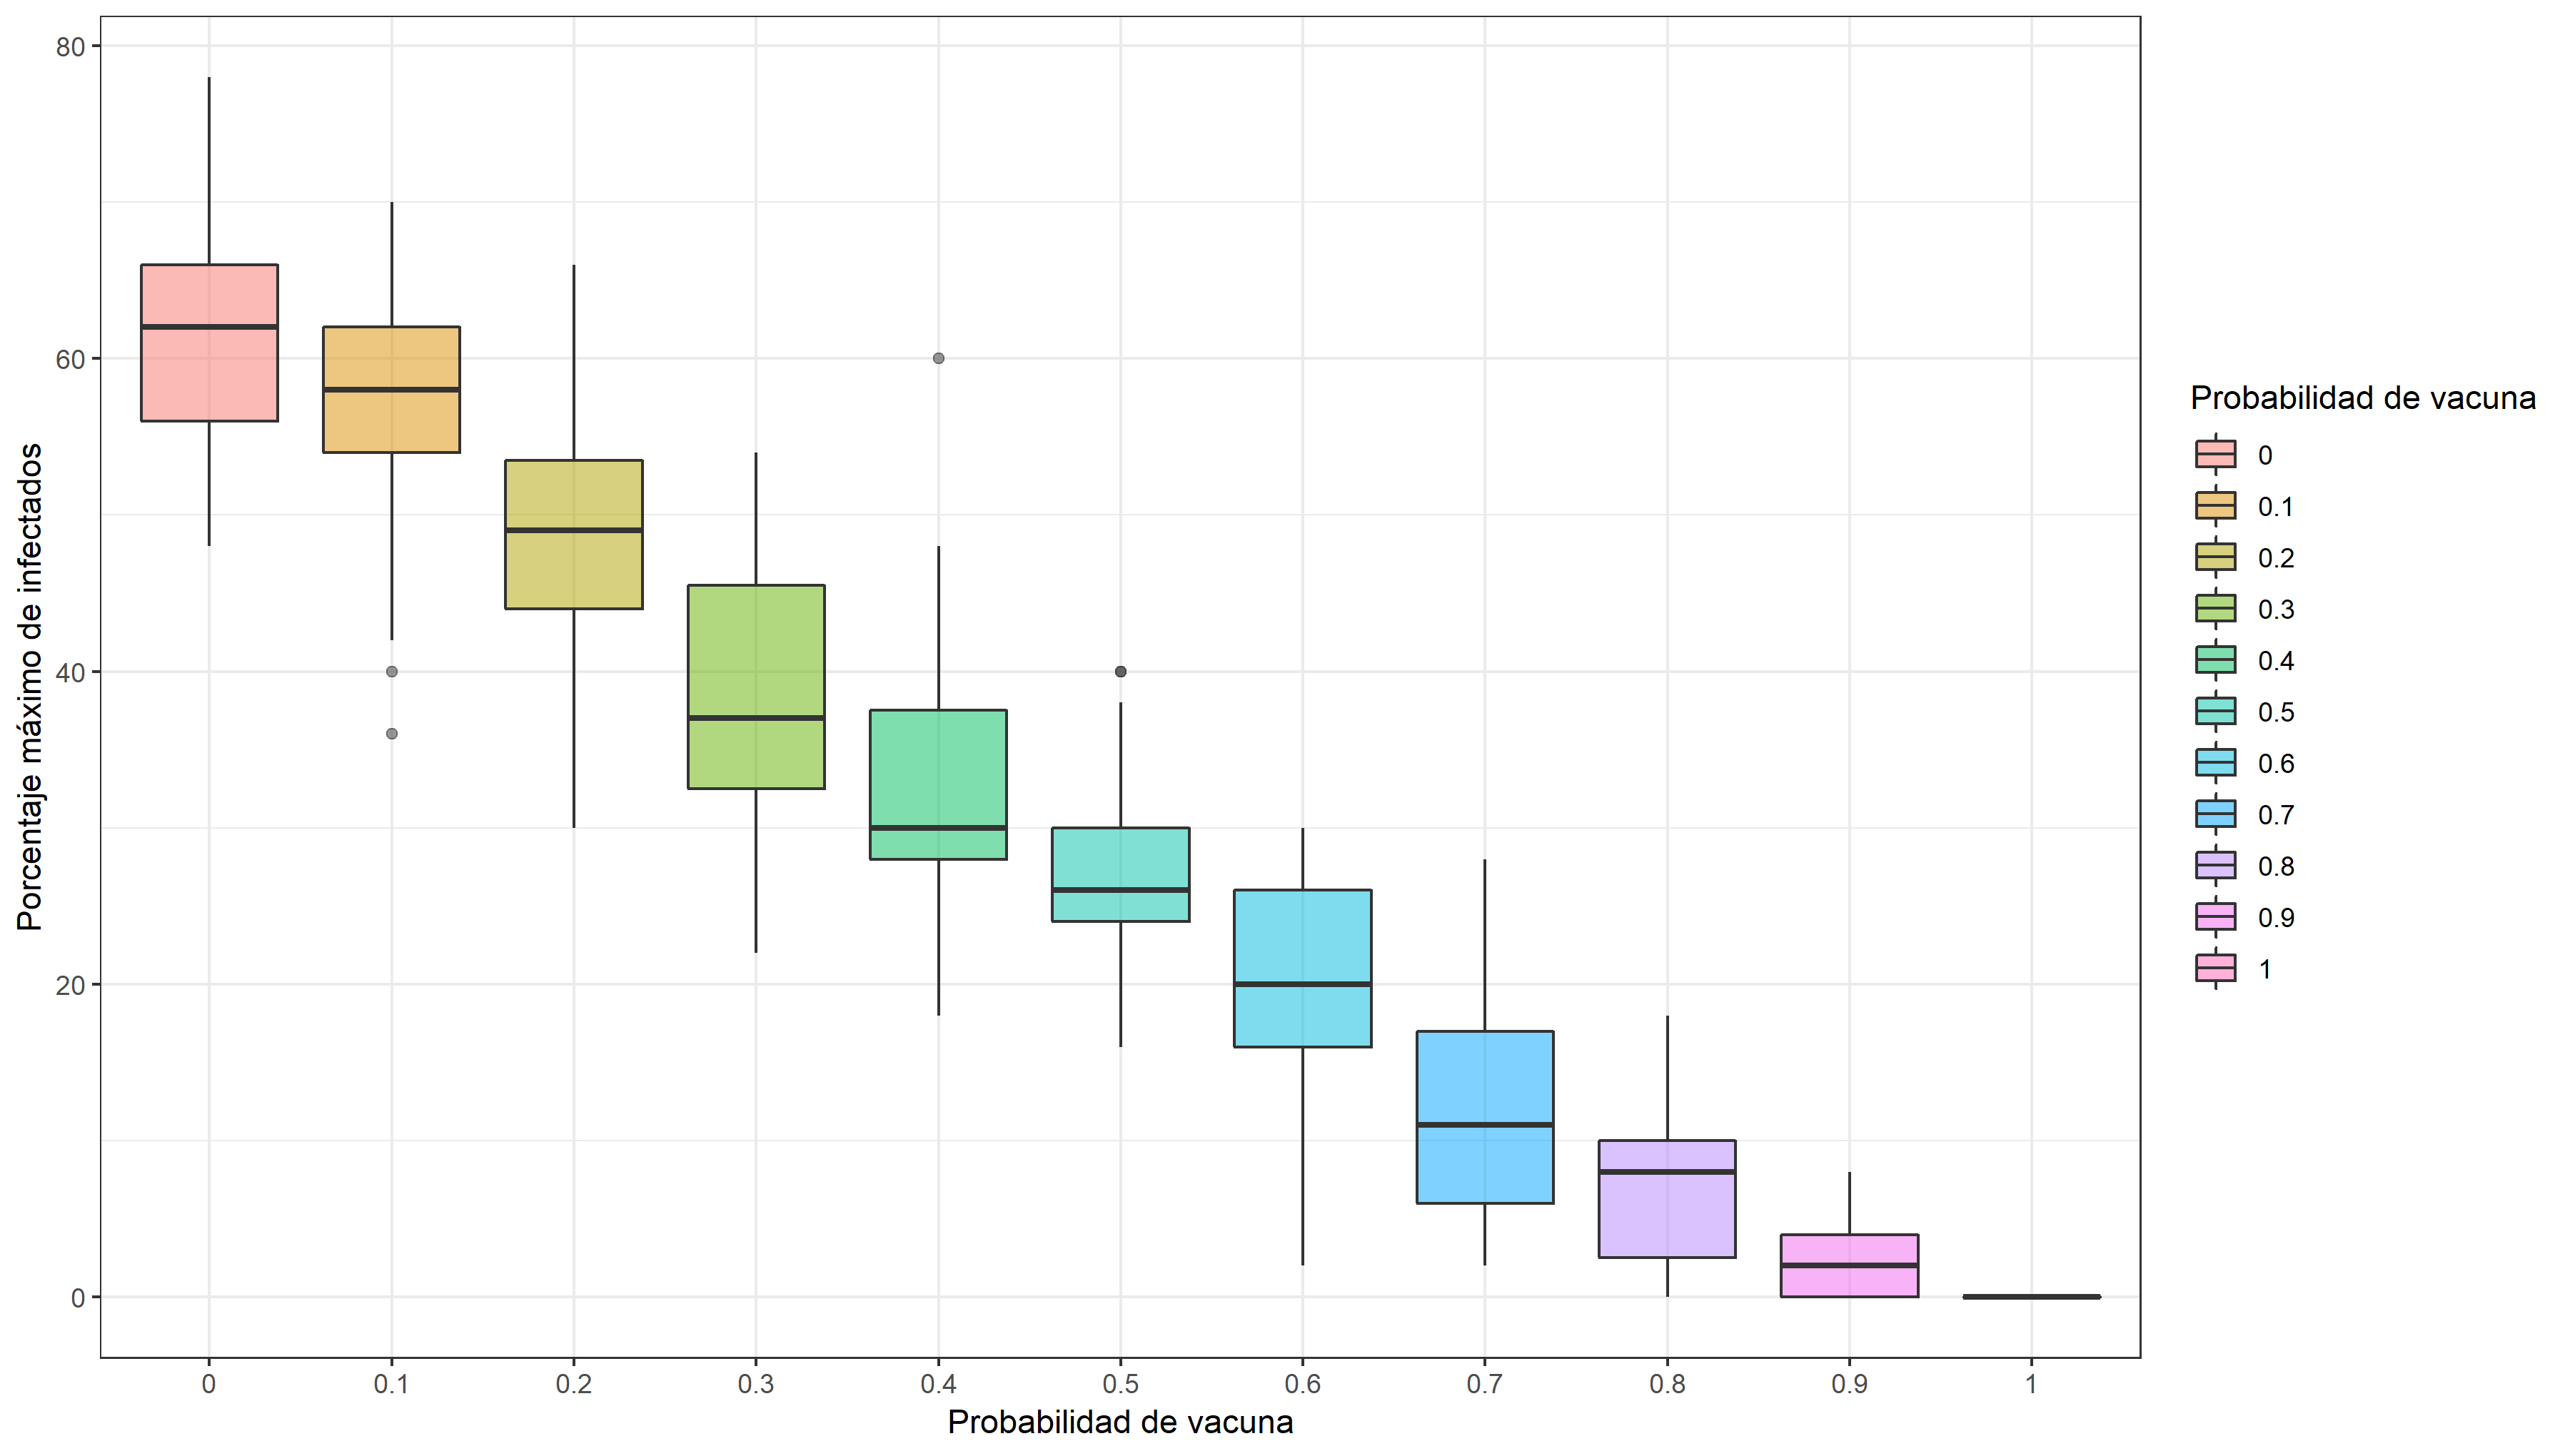
\includegraphics[width = 187 mm]{Graficap6.png}
\caption{Cambio en el porcentaje máximo de infectados con respecto a la probabilidad de generar agentes vacunados.}
\label{g1}
\end{figure}
Como se puede observar en la gráfica \ref{g1} los resultados son tal y como se esperaban, el porcentaje máximo de infectados decrece conforme la probabilidad de generar agentes vacunados aumenta.
A mayor cantidad de agentes en estado recuperados, menos posibilidad tiene los agentes con estado infectado de propagarse. 
Con una probabilidad cero la cantidad de agentes infectados recae en el movimiento de los agentes en el sistema y en la probabilidad de que se generen infectados.
Por el contrario con probabilidad uno no existe ningún agente infectado, esto es porque todos y cada uno de los agentes fueron vacunado con esta probabilidad.

\section{Primer reto}
En este reto se busca observar los cambios que existen en el porcentaje máximo de infectados al cambiar los patrones de movimiento de los agentes.

Se mantiene la modificación de las vacunas para ver la diferencia de resultados.
Se usa el modelo de punto intermedio aleatorio como base para el cambio en el patrón de movimiento en los agentes. 

Todos los agentes tienen distintas velocidades lo que significa que no todos alcanzaran su punto meta a la vez, esto se hace con el propósito de agregar más variedad al movimiento de los agentes.

Se mantienen las variaciones en la probabilidad de generar vacunados y el número de réplicas.
\lstinputlisting[language= R, firstline=6, lastline=10]{R1P6.R}
Seguido se declaran los puntos iniciales en los que aparecen los agentes y sus puntos meta, a su vez se genera un número aleatorio de pasos con el que se calcula la velocidad con la que avanza al punto meta cada agente.
\lstinputlisting[language= R, firstline=25, lastline=29]{R1P6.R}
Todo esto se genera dentro de un rango de cero a el tamaño del área en el que se mueven los agentes lo que permite omitir la transformación en toroide del área.
Para que la velocidad con la que llega al punto meta concuerde con la distancia en pasos que se recorre se realiza la siguiente operación.
\lstinputlisting[language= R, firstline=31, lastline=32]{R1P6.R}
Se calcula la diferencia entre los puntos en los que se encuentra el agente y el punto meta y seguido se divide entre el número de pasos para tener una relación que indica cuanto avanza hasta llegar al punto meta.
Esto se traduce como la velocidad con la que se traslada el agente hasta su punto meta.
\lstinputlisting[language= R, firstline=33, lastline=37]{R1P6.R}
El número de pasos sirve como contador para cambiar de punto meta una vez haya completado su recorrido al primer punto meta.
Más adelante se realiza el cambio en el movimiento de cada uno de los agentes.
Se procede a realizar los cambios de movimiento en cada paso.
\lstinputlisting[language= R, firstline=90, lastline=110]{R1P6.R}
En cada iteración el agente avanza de su posición hsata el punto meta con la velocidad antes calculada, además, se resta uno en cada paso para determinar cuando ha alcanzado su meta.
Una vez hecho esto, las posiciones iniciales de los agentes pasaran a ser los puntos meta anteriores y luego se calculan nuevos puntos meta y se calcula nueva mente la velocidad pues es una distancia distinta la que recorre ahora el agente. También se restablecen los pasos para llevar su cuenta nuevamente.

Se obtiene los resultados en la gráfica \ref{g2}.
\begin{figure}[H]
\centering
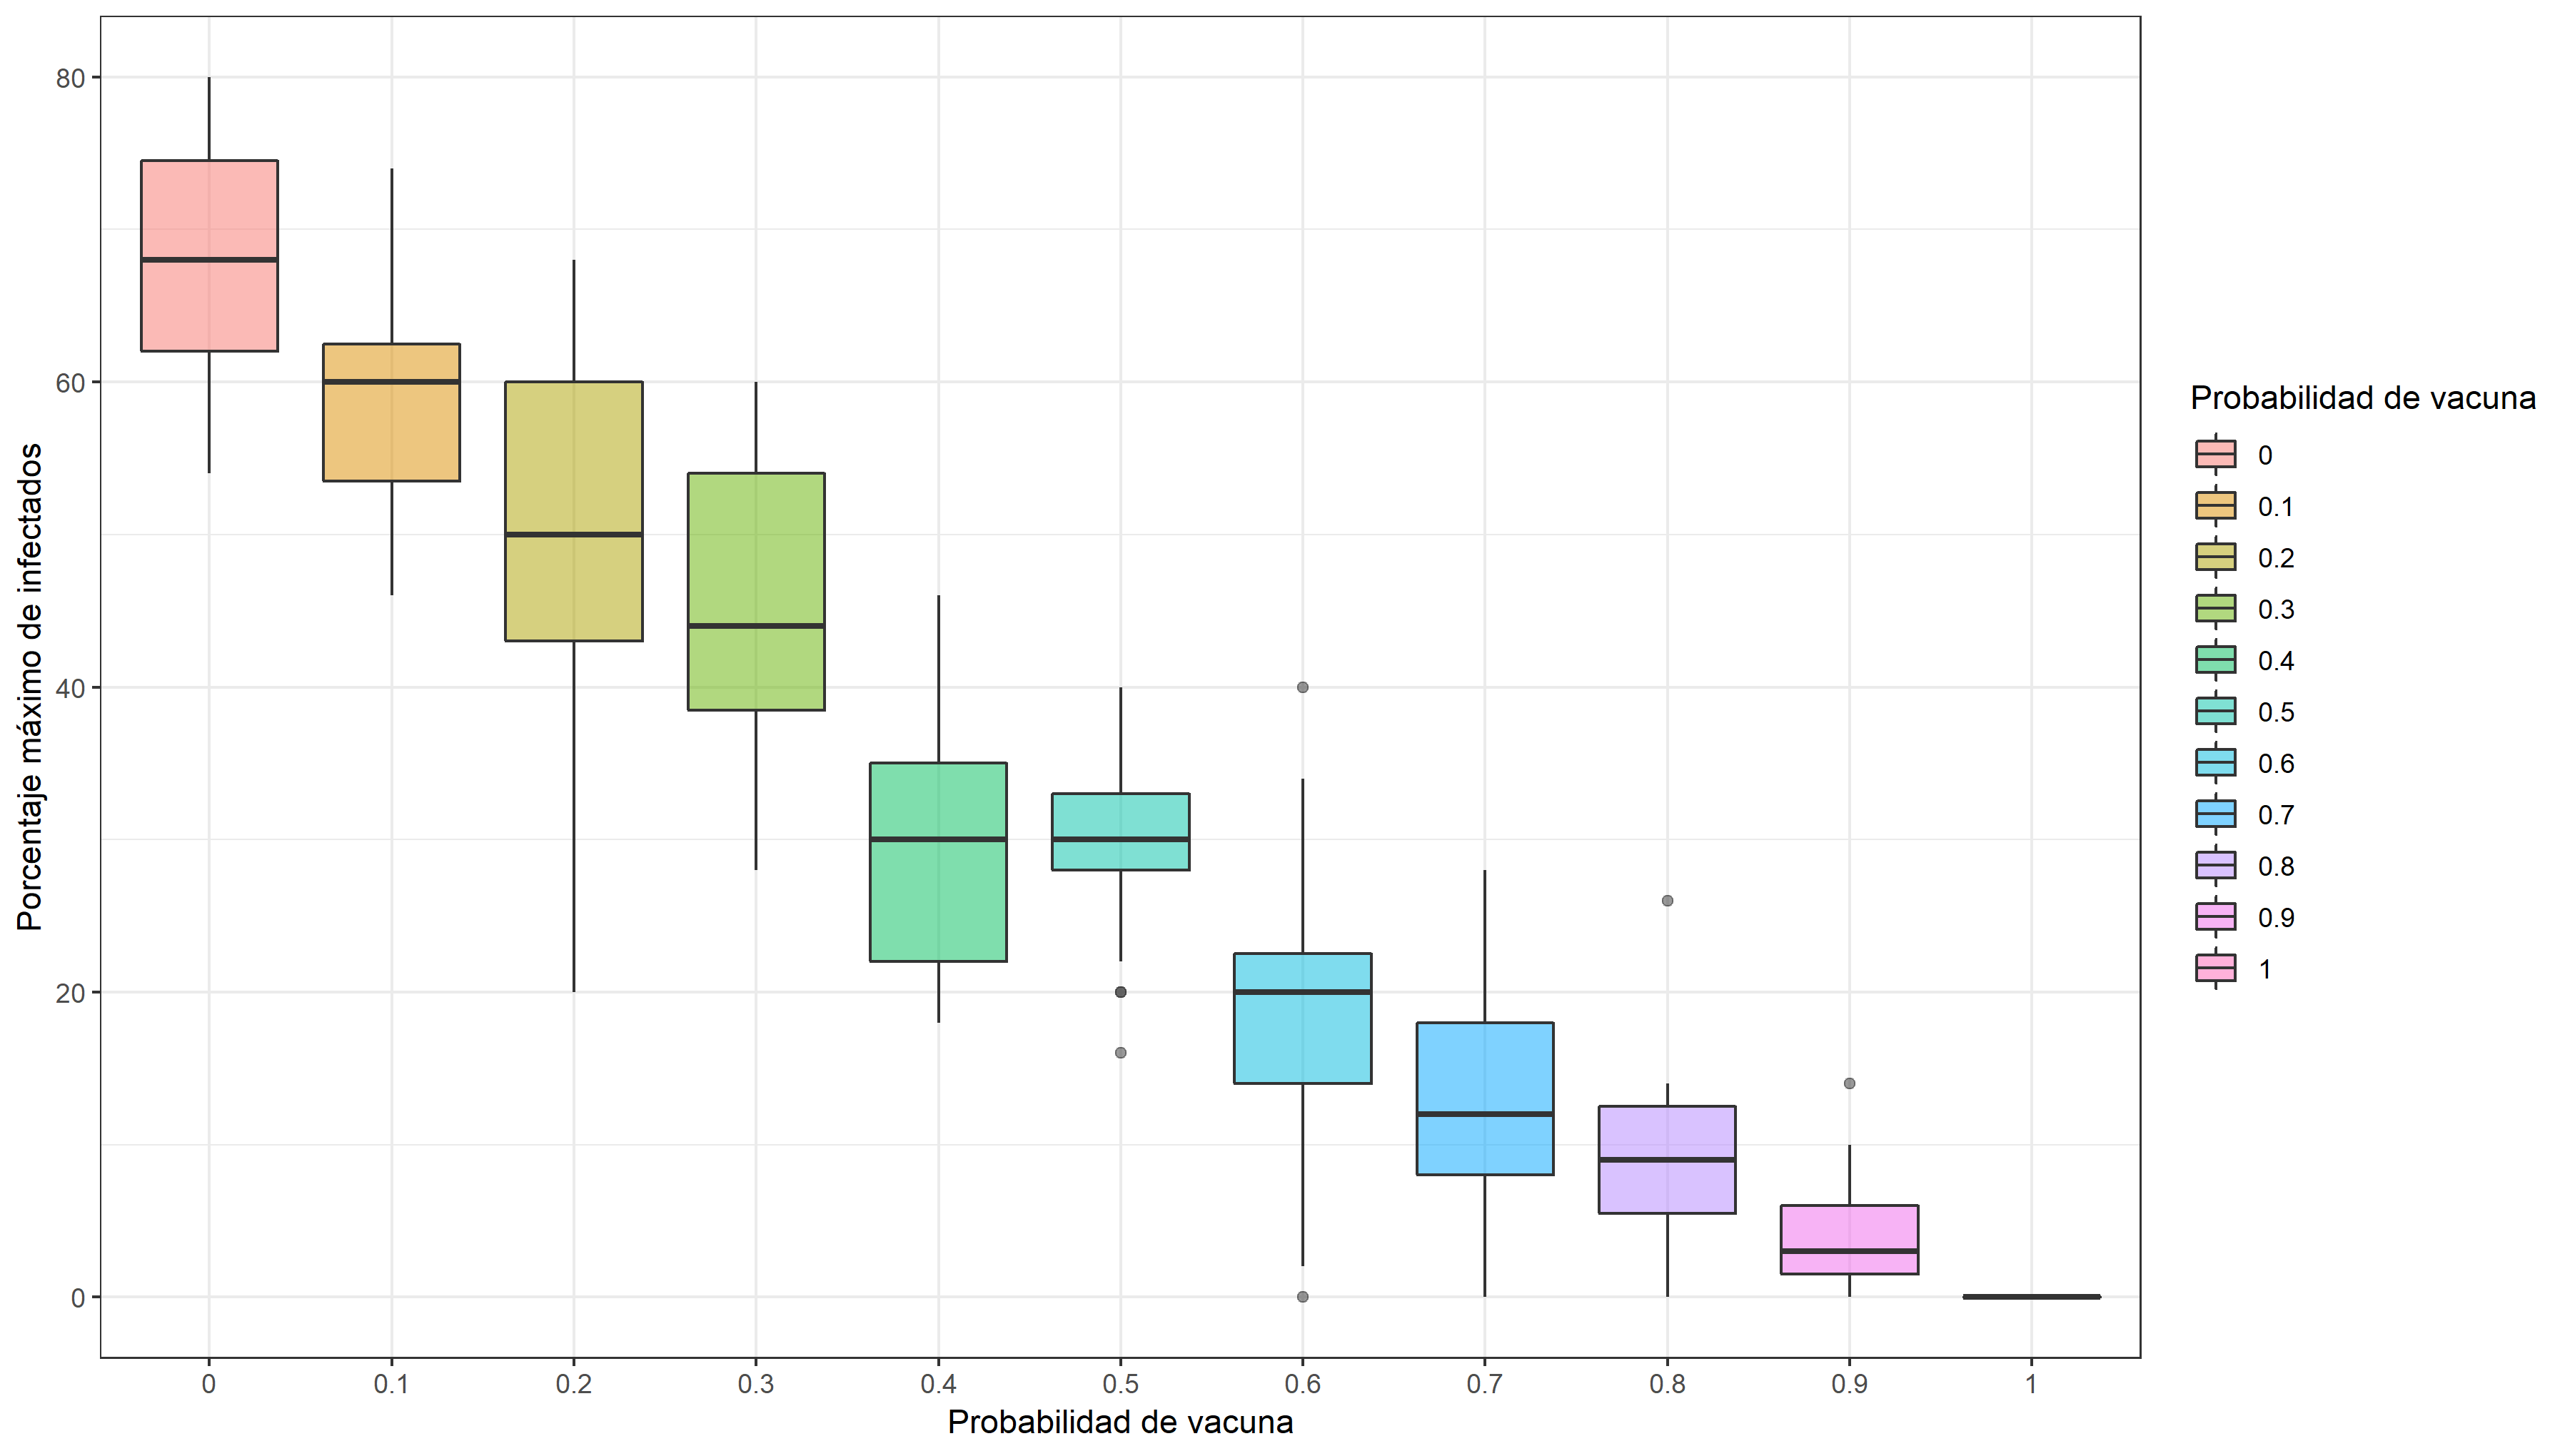
\includegraphics[width = 187 mm]{Grafica2p6.png}
\caption{Cambio en el porcentaje máximo de infectados con respecto a la probabilidad de generar agentes vacunados (modelo de punto intermedio aleatorio).}
\label{g2}
\end{figure}

Concluyendo con el reto uno, la variedad que el modelo de punto intermedio aleatorio aporta al sistema multiagente es notoria. A diferencia del sistema con trayectorias fijas, en este los agentes alcanzan más sitios del área a su vez que se cruzan con más agentes y esto aumenta la probabilidad de que los agentes en estado infectado propaguen. Con este nuevo patrón de movimiento el porcentaje de infectados ha aumentado en cada una de sus variaciones de probabilidades, a excepción del caso aislado de probabilidad uno.

\begin{thebibliography}{9}

\bibitem{r} 
R:  R Project, 2019
\\\texttt{https://www.r-project.org/}

\bibitem{satu} 
Satu Elisa Schaeffer: Práctica 6: sistema multiagente, 2019
\\\texttt{https://elisa.dyndns-web.com/teaching/comp/par/p6.html}



\end{thebibliography}










\end{document}